\subsection{Exercise 1}
($\mu$/$\rho$,$\lambda$)-ES where $\mu$ denotes the number of parents, $\rho\leq\mu$ the number of parents involved in the producing a single offspring (mixing number), $\lambda$ the number of offspring without self adaptation or recombination

\begin{itemize}
    \item What happens if you make $\lambda$ smaller e.g. $\lambda=\mu$? You select all offsprings instead of best $\mu$ individuals thus resulting in worse overall fitness. For example $\lambda=100$ and $\mu=20$ result in a best fitness value of 150 while $\lambda=100$ and $\mu=20$ results in a fitness value of 300 
    \item What happens if you increase the mixing number $\rho$? Too little parents and we aren't exploiting the genetic material of the parents enough, too many parents and we lose diversity in the population ($\rho=1 \rightarrow $ 152 best fitness, $\rho=5 \rightarrow $ 65 best fitness, $\rho=20 \rightarrow $ 108 best fitness)
    \item Does this confirm or contradict the conclusions you drew in the first module?
\end{itemize}

Self adaptation differences
\begin{itemize}
    \item Sphere: problem simple enough that individual and global adaptation yield roughly the same results
    \item Rosenbrock: global and individual adaptation yield similar result (0.58 vs 0.31 best fitness). Probably this is due to the fact that for individual adaptation all mutations rate tends to become similar when the population reaches the bottom plateau
    \item Rastrigin: global adaptation performs better than individual (9 vs 27 best fitness). Might be because the individual parameters are more prone to get stuck in local minima since the function is highly multimodal
\end{itemize}

\subsection{Exercise 2}
\subsubsection{Sphere}
\begin{figure}[H]
    \centering
    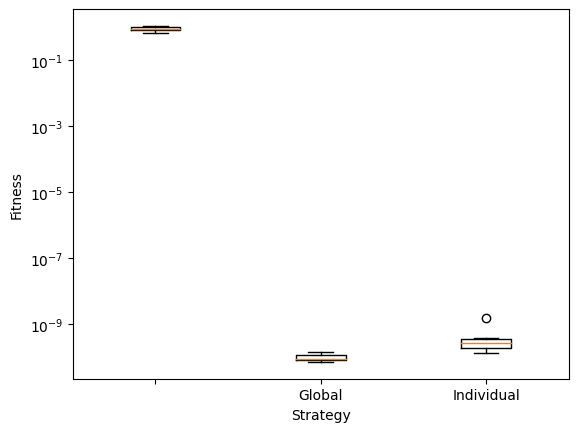
\includegraphics[width=\linewidth]{images/lab3/sph_strat.png}
\end{figure}
min fitness (no self adaptation): 0.6295797013407892 \\
min fitness (global strategy): 7.350456446289495e-11 \\
min fitness (individual strategy): 1.3420058194203682e-10 \\

\subsubsection{Rosenbrock}
\begin{figure}[H]
    \centering
    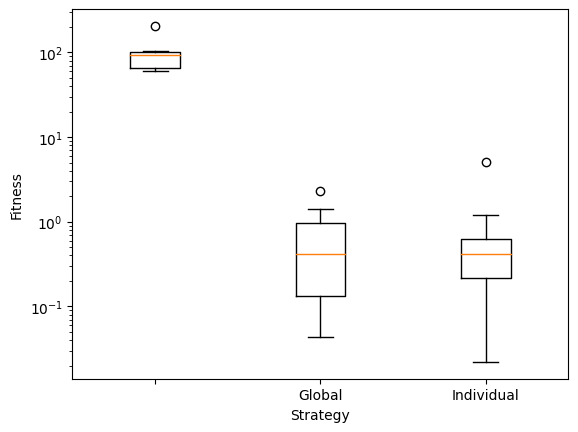
\includegraphics[width=\linewidth]{images/lab3/ros_strat.png}
\end{figure}
min fitness (no self adaptation): 60.20330481741628  \\
min fitness (global strategy): 0.04357456356967017 \\
min fitness (individual strategy): 0.022078762071256034 \\

\subsubsection{Rastrigin}
\begin{figure}[H]
    \centering
    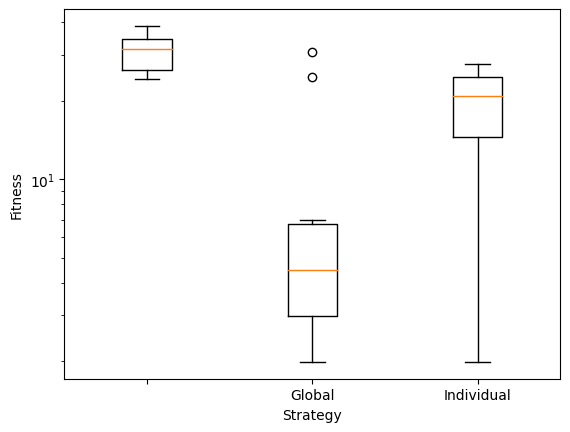
\includegraphics[width=\linewidth]{images/lab3/ras_strat.png}
\end{figure}
min fitness (no self adaptation): 24.14511286571318 \\
min fitness (global strategy): 1.9899181355932818 \\
min fitness (individual strategy): 1.9928226583738748 \\

\noindent In general we can see from the box plot that individuals created by using a global adapting strategy tends to produce individuals that are much closer together than using an individual adaptation strategy

\subsection{Exercise 3}
\subsubsection{Sphere}
\begin{figure}[H]
    \centering
    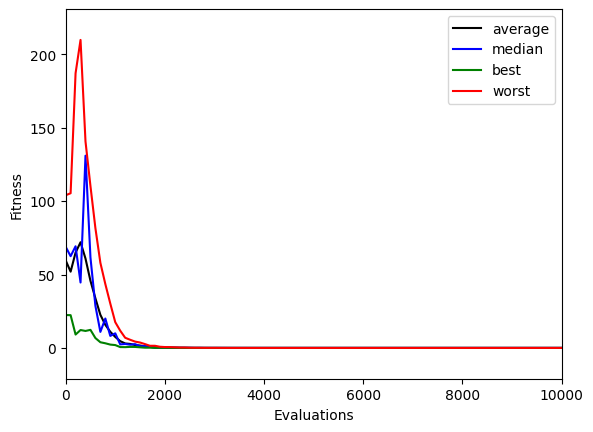
\includegraphics[width=\linewidth]{images/lab3/sph_cma.png}
\end{figure}
Best Individual: [ 3.55708404e-07  2.44509255e-07  7.68957828e-08  8.40119643e-08 5.57895771e-07 -8.61813824e-08 -1.13038822e-06 -8.82562967e-07 6.06012259e-07 -6.97759931e-07] \\
Best Fitness: 3.4287738433000135e-12

\subsubsection{Rosenbrock}
\begin{figure}[H]
    \centering
    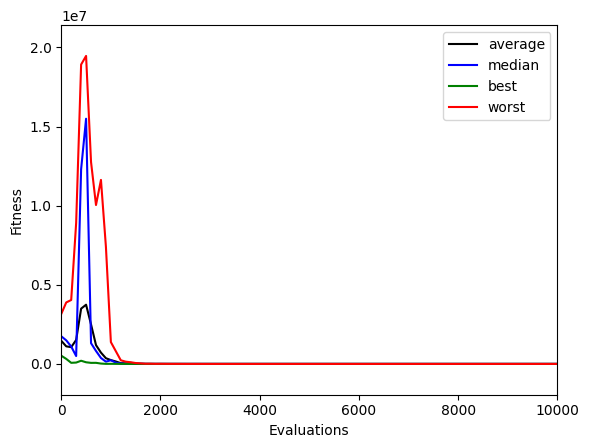
\includegraphics[width=\linewidth]{images/lab3/ros_cma.png}
\end{figure}
Best Individual: [ 0.98631674  0.96942083  0.9173355   0.86717045  0.76022123  0.58081645 0.35165418  0.11238196  0.01022353 -0.01231165] \\
Best Fitness: 2.620872257772964

Works particularly well with Rosenbrock since the covariance matrix allows the updates to be more aligned with the direction of the valley at the bottom of the function

\subsubsection{Rastrigin}
\begin{figure}[H]
    \centering
    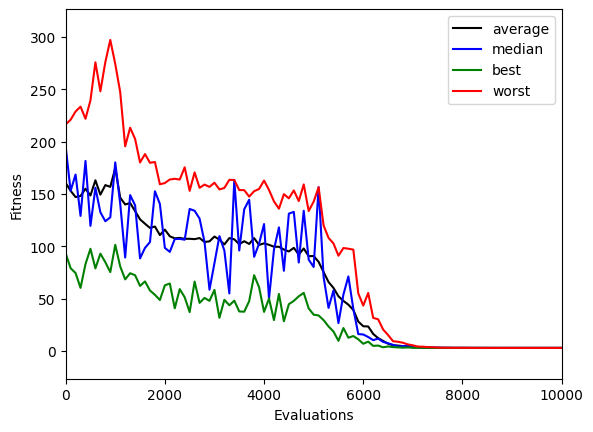
\includegraphics[width=\linewidth]{images/lab3/ras_cma.png}
\end{figure}
Best Individual: [-2.50260374e-05  2.06766433e-05  8.20034734e-05 -5.67617832e-05 9.94949458e-01  2.44508718e-04 -9.94929298e-01  9.95023360e-01 -5.32783338e-05 -7.95925573e-05] \\
Best Fitness: 2.9848940524220815

\noindent In general not only CMA finds a good approximation of the optimum but it is also very fast in doing it (the values above are the ones for 100 generations but we can achieve much better results just by doubling)

\subsection{General questions}
Do the observations you made while varying $\mu$, $\rho$, and $\lambda$ confirm or contradict the conclusions you drew in the previous module's exercises?

What are the advantages of self-adaptation in evolutionary computation?

In what ways might self-adaptation be occurring in biological organisms?

Compare the different self-adaptation strategies explored in this exercise. In what ways are certain strategies better than others for optimization? In what ways are certain strategies more biologically plausible than others?

Describe what reasons may contribute to better performance of CMA-ES and what can be the conditions when CMA-ES is not better than a basic ES.
